\documentclass[a4paper,11pt]{report}
\usepackage[T1]{fontenc}
\usepackage[english, italian]{babel}
\usepackage[utf8]{inputenc}
\usepackage[xindy]{imakeidx}
\usepackage{xcolor}
\usepackage{graphicx}
\usepackage{amsmath}
\usepackage{amssymb}
\usepackage{etaremune}
\usepackage{enumitem}
\usepackage[toc,page]{appendix}
\usepackage{verbatimbox}
\usepackage{amsthm}

\theoremstyle{plain}
\newtheorem{thm}{Teorema}[section]

\usepackage[hidelinks, colorlinks=true]{hyperref}	
\usepackage{bookmark}
\usepackage{caption}
\usepackage{subfig}

\captionsetup{tableposition=top, figureposition=bottom, font=small}
\setcounter{tocdepth}{3}
\setcounter{secnumdepth}{3}


\usepackage{epigraph}


\makeindex


\includeonly{
			Sezioni/Introduzione,
			Sezioni/DFA,
			Sezioni/NFA,
			Sezioni/EspressioniRegolari
			}		
		
\begin{document}

\title{Automi e Linguaggi Formali}
\author{Sara Feltrin}
\date{26-02-18}

\maketitle



\newpage

\hypersetup{linkcolor=blue, urlcolor=blue}

\chapter{Introduzione}
Per iniziare, ci sono alcuni concetti di base da tenere a mente:

\begin{itemize}

\item \textbf{Alfabeto}: insieme finito e non vuoto di simboli, per esempio
$\Sigma$ = \{0,1\} oppure $\Sigma$ = \{a,b,c,d,e,..,z\};
\item \textbf{Stringa}: sequenza finita di simboli da un alfabeto $\Sigma$, per 
esempio: 011001 o abc;
\item \textbf{Stringa vuota}: stringa con zero occorrenze di simboli dell'alfabeto 
$\Sigma$, denotata da $\varepsilon$;
\item \textbf{Lunghezza di una stringa}: numero di simboli nella stringa, per 
esempio $|$w$|$ denota la lunghezza della stringa w, quindi $|$01001$|$ = 5;
\item \textbf{Potenze di un alfabeto}: $\Sigma^{k}$ insieme delle stringhe di 
lunghezza k con simboli da $\Sigma$, per esempio preso l'alfabeto $\Sigma$=\{0,1\}:
$\Sigma^{0}$=\{$\varepsilon$\}, $\Sigma^{1}$=\{0,1\}, $\Sigma^{2}$=\{00,01,10,11\}.
Viene chiamata potenza di un alfabeto poichè può essere vista come una potenza dove 
la base è il numero di simboli dell'alfabeto e l'esponente il numero della potenza
dell'alfabeto (quindi, nell'alfabeto dei numeri binari con $\Sigma^{3}$, avremo
 $2^{3}=8$);
\item \textbf{Insieme di tutte le stringhe}: per ottenere l'insieme di tutte le 
stringhe, usiamo il simbolo \textbf{*} e scriviamo $\Sigma^{*}=\Sigma^{0} \cup 
\Sigma^{1} \cup \Sigma^{2} \cup ..$ ;
\item \textbf{Linguaggio}: dato un alfabeto $\Sigma$, chiamiamo linguaggio ogni
sottoinsieme $L\subseteq\Sigma^{*}$ (compreso anche il linguaggio vuoto che non 
contiene nessuna parola).

\end{itemize}

\chapter{Automi a stati finiti deterministici}
Un automa a stati finiti deterministico, chiamato anche DFA, è una quintupla
$A=(Q, \Sigma, \delta, q_0, F)$ dove
\begin{itemize}
\item Q è un insieme finito di stati;
\item $\Sigma$ è un alfabeto finito, si intende quindi l'insieme di
input che può leggere l'automa;
\item $\delta$ è una funzione di transizione $(q,a) \mapsto q'$, ovvero 
dallo stato in cui sono, quando leggo il simbolo a, passo allo stato $q'$;
\item $q_0 \subseteq Q$ è lo stato iniziale dell'automa;
\item $F \subseteq Q$ è un insieme di stati finiti;
\end{itemize}
L'automa può essere rappresentato sia come diagramma di transizioni sia come tabella
di transizioni: 

\begin{figure}[h]
\centering 
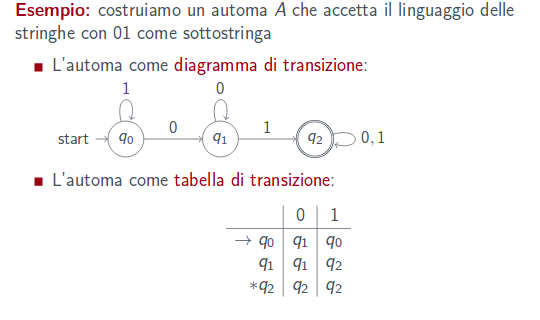
\includegraphics[scale=0.5]{Immagini/DFA.png}
\end{figure}

\section{Linguaggio accettato da un DFA} 
La funzione di transizione prende in input uno stato e una parola dando in output
una nuova parola. Definizione:
\begin{itemize}
\item \textbf{base}: $\delta(q,\varepsilon)=q \rightarrow$ ritorna lo stadio in cui è;
\item \textbf{induzione}: $\widehat{\delta}(q,w)=\delta(\widehat{\delta}(q,x),a)$, 
dove $\widehat{\delta}$ rappresenta lo stato attuale e $\delta$ lo stato in cui mi 
troverò, a indica l'ultima lettera della parola che voglio leggere.
NB: in $\widehat{\delta}$ faccio la ricorsione fino ad arrivare al caso base;
\end{itemize}
Detto ciò, possiamo definire il linguaggio accettato da A in questo modo:
$L(A)=\{w: \widehat{\delta}(q_0,w) \in F\}$. Tutti i linguaggi accettati da DFA 
vengono chiamati \textbf{linguaggi regolari}.
\chapter{Automi stati finiti non deterministici}
È un automa che può trovarsi contemporaneamente in più stati diversi e le 
transizioni non devono per forze essere complete, per esempio: 

\begin{figure}[h]
\centering 
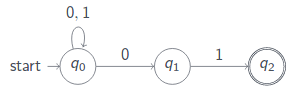
\includegraphics[scale=0.5]{Immagini/NFA.png}
\end{figure}

Infatti questo non può essere un DFA perchè da $q_0$ se leggo 0 posso trovarmi
contemporaneamente in $q_0$ e $q_1$, in più da $q_1$ posso muovermi solo in $q_2$ 
e da $q_2$ non posso proprio muovermi.
Un automa a stati finiti non deterministici(NFA) è una quintupla $A=(Q, \Sigma, 
\delta, q_0, F)$ dove
\begin{itemize}
\item Q è un insieme finito di stati;
\item $\Sigma$ è un alfabeto finito;
\item $\delta$ è una funzione di transizione che prende in input (q,a) e 
restituisce un sottoinsieme di Q;
\item $q_0 \in Q$ è lo stato iniziale;
\item $F \in Q$ è un insieme di stati finali;
\end{itemize}
Anche per i NFA abbiamo una definizione rigorosa:
\begin{itemize}
\item \textbf{base}: $\widehat{\delta}(q, \varepsilon)={q}$;
\item \textbf{induzione}: $\widehat{\delta}(q,w)=\bigcup_{p \in \delta 
(\widehat{q},x)}^{} \delta(p,a)$;
\end{itemize}
Data una parola, il nostro automa potrà trovarsi in uno dei tanti stati
che siamo andati a calcolare.

\section{Equivalenza tra DFA e NFA}
NFA e DFA sono in grado di riconoscere gli stessi linguaggi e l'equivalenza si
dimostra mediante una \textbf{costruzione a sottoinsiemi}. Infatti, dato un NFA
$N=(Q_N, \Sigma, q_0, \delta_N, F_N)$ costruiremo un DFA $D=(Q_D, \Sigma, {q_0}, 
\delta_D, F_D)$ tale che L(D)=L(N).
Ogni stato del DFA, $Q_D$ corrisponde ad un insieme di stati dell'NFA.
\textit{Uno stato del DFA $F_D$ è finale se c'è almeno uno stato finale
corrispondente all'NFA}. La funzione di transizione $\delta_D$ percorre tutte le
possibili strade. Ad esempio: 

\begin{figure}[h]
\centering 
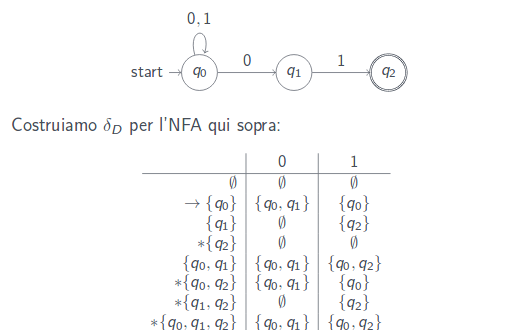
\includegraphics[scale=0.5]{Immagini/equivalenza1.png}
\end{figure}

\begin{figure}[h]
\centering 
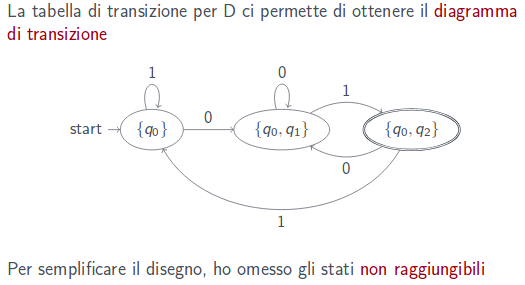
\includegraphics[scale=0.5]{Immagini/equivalenza2.png}
\end{figure}

\begin{thm}
Sia D il DFA ottenuto da un NFA N con la costruzione a sottoinsiemi. Allora
L(D)=L(N).
\end{thm}

\begin{thm}
Un linguaggio L è accettato da un DFA se e solo se è accettato da un NFA.
\end{thm}




















\chapter{Espressioni regolari}
Diciamo che una parola è accettata oppure no in base allo stato in cui giungiamo alla
fine di questa parola (se sono in uno stato finale, allora si tratta di una parola accettata
dall'automa altrimenti no).
Un'espressione regolare è un modo dichiarativo per descrivere un linguaggio regolare.
Abbiamo diversi tipi di operazioni sui linguaggi:

\begin{itemize}
\item \textbf{Unione}: $L\cup M=\{w:w \in L oppure w \in M\}$
\item \textbf{Concatenazione}: $L.M=\{uv : u \in L e v \in M\}$
\item \textbf{Potenze}: 
	\begin{itemize}
	\item $L^{0}=\{\varepsilon\}$
	\item $L^{1}=L$   
	\item $L^{k}=L.L...L(k volte)$
	\end{itemize}
\item \textbf{Chiusura di Kleene}: $L^{\ast} = \bigcup_{i=0}^\infty L^{i}$
\end{itemize} 

Inoltre le espressioni regolari sono costruite utilizzando 

\begin{itemize}
\item un insieme di costanti di base:
	\begin{itemize}
	\item $\varepsilon$ per la stringa vuota
	\item $\emptyset$ per il linguaggio vuoto
	\item a,b,.. per i simboli $a,b,..\in \Sigma$
	\end{itemize}
\item collegati da operatori:
	\begin{itemize}
	\item $+$ per l'unione;
	\item $\cdot$ per la concatenazione;
	\item $\ast$ per la chiusura di Kleene;
	\end{itemize}
\end{itemize}

Esistono anche delle \textbf{regole di precedenza} degli operatori:
\begin{itemize}
\item[1]Chiusura di Kleene;
\item[2]Concatenazione;
\item[3]Unione.
\end{itemize}

\section{Equivalenza tra FA e RE}
DFA, NFA e $\varepsilon$\textrm{-NFA} sono tutti equivalenti.

\begin{figure}[h]
\centering 
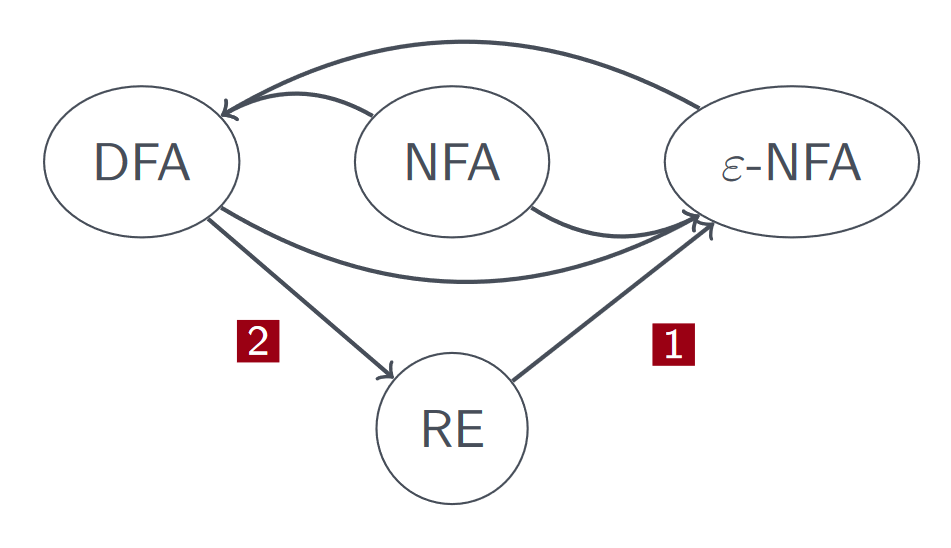
\includegraphics[scale=0.5]{Immagini/equivalenza3.png}
\end{figure}

Infatti 
\begin{itemize}
\item[1] Per ogni espressione regolare \textbf{R} esiste un $\varepsilon$\textrm{-
NFA}A, tale che L(A)=L(\textbf{R});
\item[2] Per ogni FA A possiamo costruire un'espressione regolare \textbf{R},
tale che L(\textbf{R})=L(A).
\end{itemize}

\section{Conversione per eliminazione di stati}
Quando uno stato \textbf{q} viene eliminato, i cammini che passano per q scompaiono.
Quindi si aggiungono nuove transizioni etichettate con espressioni regolari che 
rappresentano i cammini eliminati. Alla fine otteniamo un'espressione regolare che
rappresenta tutti i cammini dallo stato iniziale ad uno stato finale, ovvero
\textbf{il linguaggio riconosciuto dall'automa}.








\end{document} 